\documentclass[11pt,twocolumn]{article}
\setlength{\columnsep}{2em}
\usepackage{times}
\usepackage{graphicx}
\usepackage{amssymb}
\usepackage{url,hyperref}

\usepackage{amsmath}
\usepackage{graphicx}
\usepackage{float}
\usepackage{makecell}

\begin{document}

\title{CSCI 5352 Project\\
Senatorial Career Archetypes and Bipartisan Voting}

\author{Andrew Guttman}

\maketitle
\thispagestyle{empty}

\begin{abstract}
A popular topic in political discussion is that of party polarization, where party positions become more and more extreme, leaving little agreed upon. This is generally considered an unfavorable trend leading to deadlock in governing processes. One way of observing this polarization is by viewing voting results of representative bodies and seeing how the "for" and "against" votes conform to party lines. In this study we observe United States Senate votes from the 115th session of congress (January 3, 2017, to January 3, 2019) to find when this trend in bucked, when there is both bipartisan support and bipartisan opposition on a vote, and attempt to determine if there is any similarity in pre-senatorial career histories from Senators who crossed party lines to vote the same that might explain this atypical behavior. Unfortunately, we do not find significant evidence that career history has an effect on these votes.
\end{abstract}

\section{Introduction}
As discussed, political polarization is generally considered negative. By finding examples when this polarization is overcome, we might identify patterns that correspond to bipartisan agreement. The possible pattern being considered in this study is career history; whether similar careers before being a Senator might influence people to a certain type of agreement on issues despite the general position taken by the Senator's political party.
	
In order to answer the question of whether or not similar career history corresponds with crossing party lines to vote in a similar fashion to others with a similar history, we first need to identify what similar career history means. Here we will gather data about the Senators serving in the 115th congress, categorize the major occupations they had before joining the Senate and create links between Senators that shared positions in the same category. With this network of Senators and the jobs that join them, we will attempt to find communities of similar career paths, coming up with some number of archetypal senatorial careers.
	
With these career archetypes, we can then identify key votes that demonstrate the desired bipartisan qualities we are looking for and see if the Senators who cast those votes belong to the same archetypes. If so, this would suggest that certain archetypal careers are either selected by, or influence someone to, a certain type of non-partisan thinking about specific issues.

\section{Data}
Data for the Senators of the 115th congress was gathered from the Wikipedia page "List of current United States senators", (archived from December 29th, 2018) including name, party affiliation and occupational history including previous offices. While Wikipedia is crowd-sourced and thus unaccountable and prone to error, the simple factual information of such public and highly scrutinized figures was assumed to be accurate enough for our purposes. Since there was turnover during the course of the 115th session of congress, data on five Senators, Jeff Sessions, Al Franken, Luther Strange, Thad Cochran and John McCain, was not included on the page and was assembled by hand from each respective person's Wikipedia page.
	
The non-profit online political encyclopedia Ballotpedia was used to identify votes to be considered in the study. Ballotpedia reports itself to be non-partisan and is written and maintained by a staff and researchers. They themselves identify 42 senatorial votes as important to understanding Senator's positions during the 115th congress on the page "Key votes: 115th Congress, 2017-2018" defining the term key votes as "votes that help citizens understand where their legislators stand on major policy issues." Of these votes, nine were selected for having bipartisan majority votes and bipartisan minority dissenting votes. Once these nine votes were identified, the actual voting records were retrieved from Congress.gov, the official online records of the proceedings of congress.
	
	\section{Methods}
With this data, we need to extract the key pieces of information. This information comes in two ways, job history and voting history.

	\subsection{Jobs}
The 105 people who served on the Senate of the 115th congress together had 91 unique job titles in the data for occupations, excluding the various public offices each might have held. In order to facilitate the construction of archetypal pre-Senate careers, categories of jobs needed to be made so that similar jobs with different titles could be grouped together. To this end 18 categories were decided on by human judgment from simply looking though all the listed jobs. The legitimacy of the following analysis is contingent on the legitimacy of the categorization, so the categories and explanations/justifications are given in detail:

\begin{enumerate}
\item Academic: Those teaching or conducting research at universities.

\item Administrative: Those holding some sort of public but non-elected office that oversees and regulates important affairs. Could reasonably be called a bureaucrat, but that phase has a certain political charge this is not intended to be invoked.

\item Agricultural: Those who has listed occupations of "farmer", "rancher" or something similar. The exact nature of the work was not investigated and thus left to it's own category as being a farmer might mean working land to simply owning it and could not be fit into the appropriate category corresponding to that relation.

\item Business: Any type of officer or executive position in the private sector when not explicitly involved with the creation of the company worked for.

\item Consultant: Due to the vagueness and potentially far reaching work of consulting, all consultant jobs where put here regardless of specialty.

\item Entrepreneurial: Those explicitly involved in the founding, owning and funding of companies.

\item Finance: Jobs around banking, trading and advising on trading.

\item Law: Lawyers and judges.

\item Media: Those involved in the creation of media, be it journalistic, artistic, commercial, etc.

\item Medical: Doctors and surgeons.

\item Military: Any type of military service. Any branch, officer, enlisted, active or reserve.

\item Nonprofit: Administrative or executive positions in the nonprofit sector.

\item Political: Staffers/advisers for office holders or any type of campaign work when not the candidate. 

\item Professional: Educated jobs general considered steady careers not covered specifically by another category. Examples include accounts, teachers.

\item Real estate: Developing and brokering real estate.

\item Religious: Missionary or pastoral job.

\item Trade: Skilled but not necessarily educated work. Craftsmen.

\item Previous elected office: Any type of public elected office.
\end{enumerate}

Other considerations could have been made, for example, type of elected office, (executive, legislative), level of governance (city, state, national), but this is what was decided on. Given the overwhelming prevalence of Senators holding previous offices, (all but four did) there was worry that these office connections would overpower other underlying structures when attempting community detention. Because of this all following analysis took two branches, considering previously held office and not considering previously held office.

With job categories fixed, a bipartite network was created with two types of nodes, Senators and job categories. Edges where drawn between nodes if a Senator had ever held a job corresponding to a job category. Multi-edges were not considered. Once the bipartite network was created, it was one-mode projected. This creates a network of Senators as nodes and edges between Senators representing that they both worked a job in the same category.

With this network of Senators we attempt to find any underlying community structure. To this end, we implemented an efficient greedy agglomerative algorithm to maximize modularity. That is, it tries to create groups in the network that have a high destiny of edges that go from a node in the group to another node in the group and a low destiny of edges going from nodes across groups. While this is typically applied to social networks of some kind where there is assumed to be a community structure, there is nothing stopping us from applying this technique to try to unveil community structure hidden in something not traditionally considered a community. With these community divisions found we can then look at voting records to determine if Senators votes have any correspondence.

	\subsection{Votes}
Selecting what votes to look at is itself an important process. Here, we decided to find votes where there is a bipartisan majority vote coupled with a bipartisan minority vote. (For this study, we are considering the two independent Senators Bernie Sanders and Angus King as Democrats, the party both caucus with.) The reason we are interested in this class of votes in particular is because of what they represent in the political context.

Votes that have a bipartisan majority are typically procedural in nature and relatively noncontroversial. When someone votes against these, there is little chance that the vote will fail and the Senator knows this. The assumption we are making is that they are not trying to stop the resolution, but trying to make a point. If Senators from opposing parties cross the party consensus on the same vote, we are making a simplifying assumption that they are making the same or related points, thus are roughly aligned in a specific issue in a way that ignores party orthodoxy. While it would also be valid to look at votes where a clear party line exists and a small contingent of one party votes with the other, we make the claim by human observation that this usually happens on highly controversial votes and thus might to subject to other pressures and political calculations, such as riding a trend of outrage to vote with the other side in an attempt to appear moderate, rather than internal drivers that we are attempting to get at with our selection criteria.

Once these votes are identified, those bipartisan dissenting votes can be compared to the community groups formed through job history to see if any groups are over represented. With this data, it is also easy to find which Senators never voted against party in this set of votes and identify if they tend to come from particular groups.

	\section{Results}
Modularity maximization does find what appear to be reasonable communities among Senators organized by job history, both when taking previous office into account [fig1, 3] and not [fig2, 4].

Each partitions Senators into four communities. The character of the communities and the Senators that make them up can be found in figures 2 and 3.
	
\begin{figure}[H]
    \centering
    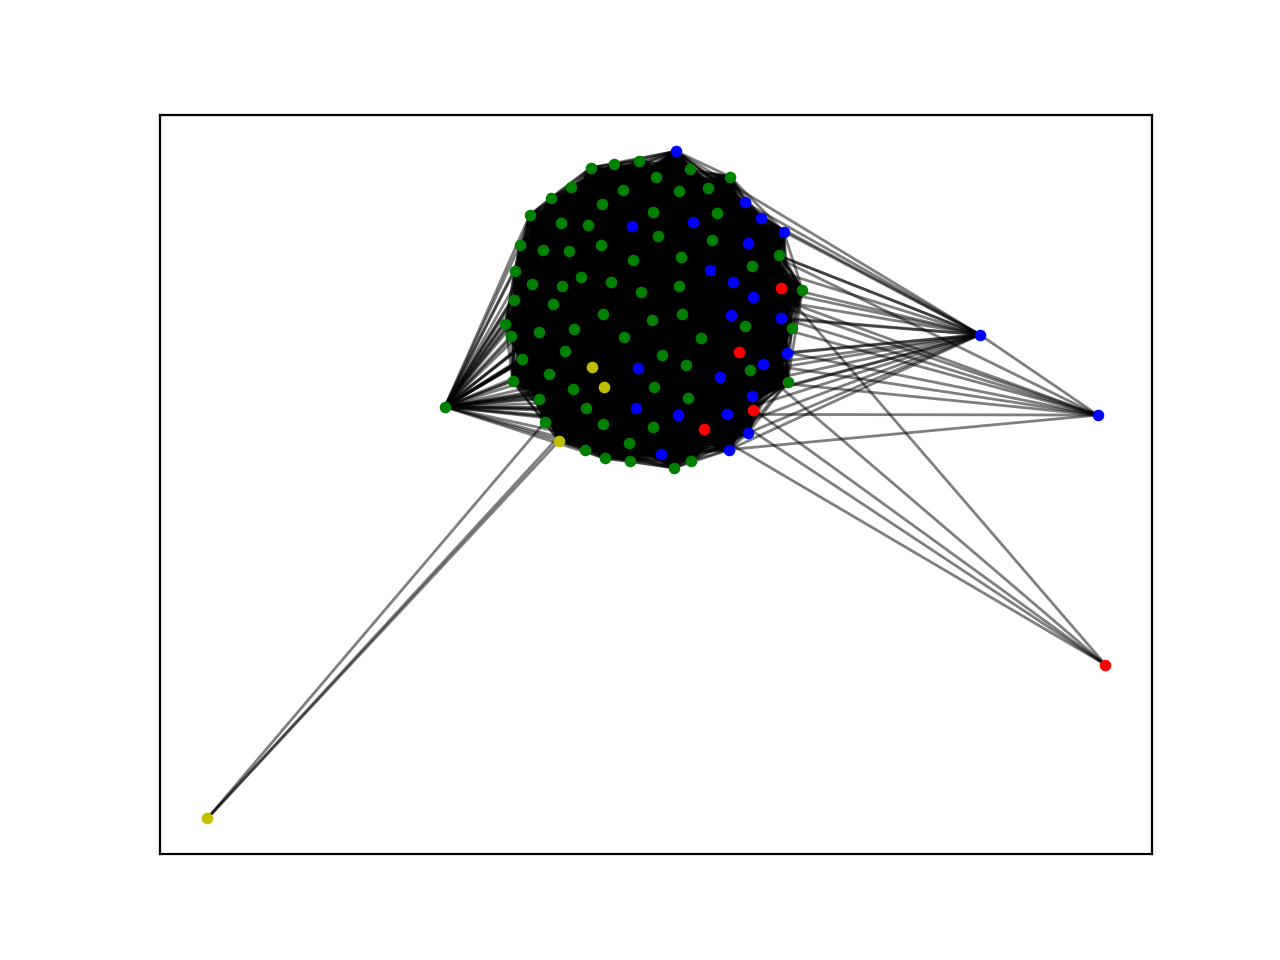
\includegraphics[width=2.5in]{comm_dis_w_office}
    \caption{{Community structure of Senator network when considering previous office. Left unlabeled to give intuitive visual aid. Details in fig 3.}}
    \label{fig:ds}
\end{figure}

\begin{figure}[H]
    \centering
    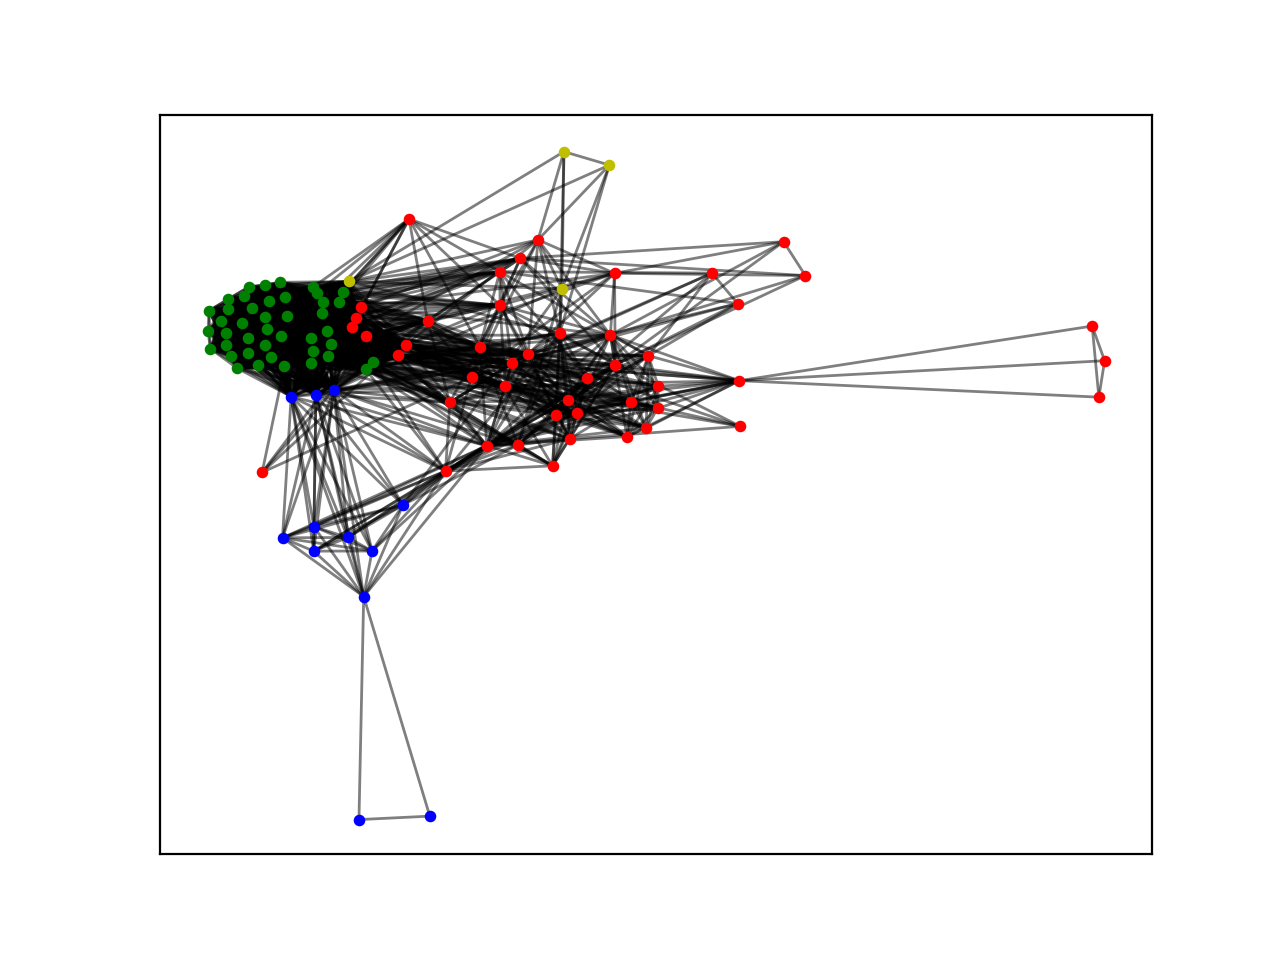
\includegraphics[width=2.5in]{comm_dis_no_office}
    \caption{{Community structure of Senator network when not considering previous office. Left unlabeled to give intuitive visual aid. Details in fig 4.}}
    \label{fig:ds}
\end{figure}

\begin{figure}[H]
    \centering
    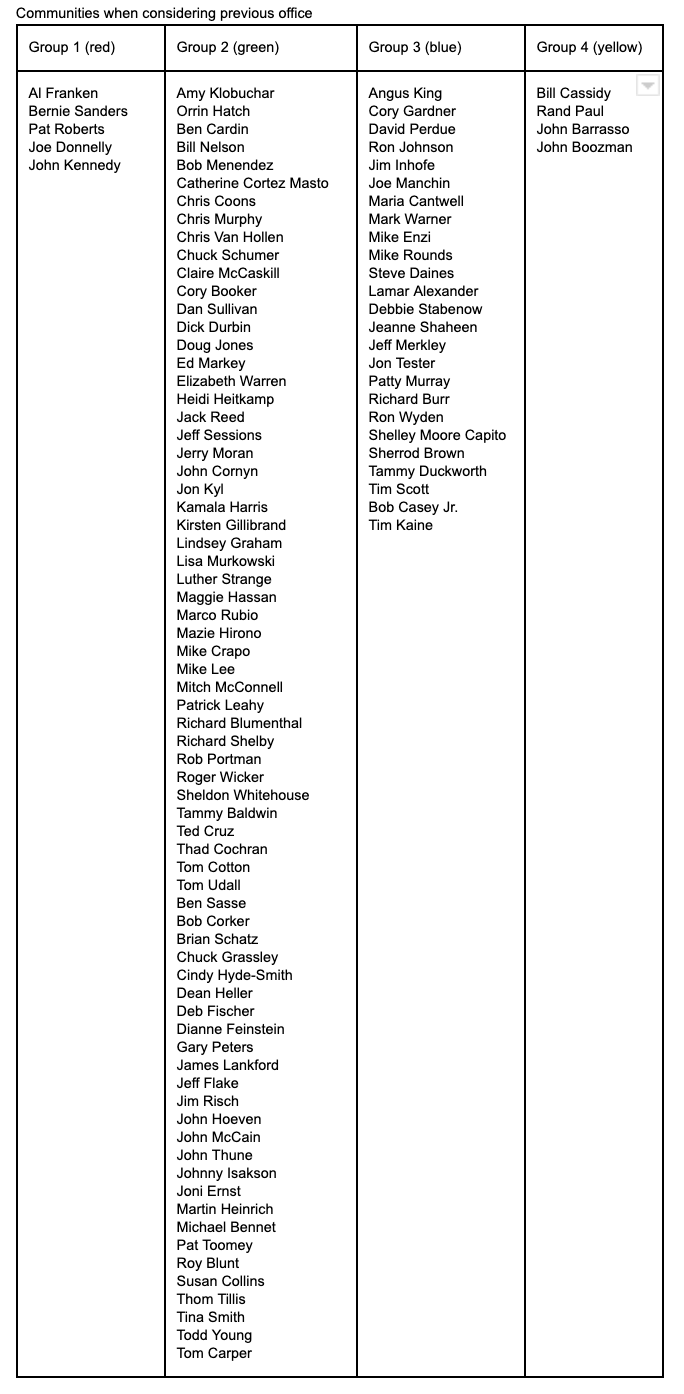
\includegraphics[width=3.2in]{comm_office}
    \caption{Communities of Senators by career history when considering previous office. \newline Group 1 is characterized by careers that included media. \newline Group 2 is characterized by careers that focus almost exclusively on law. \newline Group 3 is characterized by a mix of business and professional careers. \newline Group 4 is characterized by careers that focus almost exclusively on medicine.}
    \label{fig:ds}
\end{figure}

\begin{figure}[H]
    \centering
    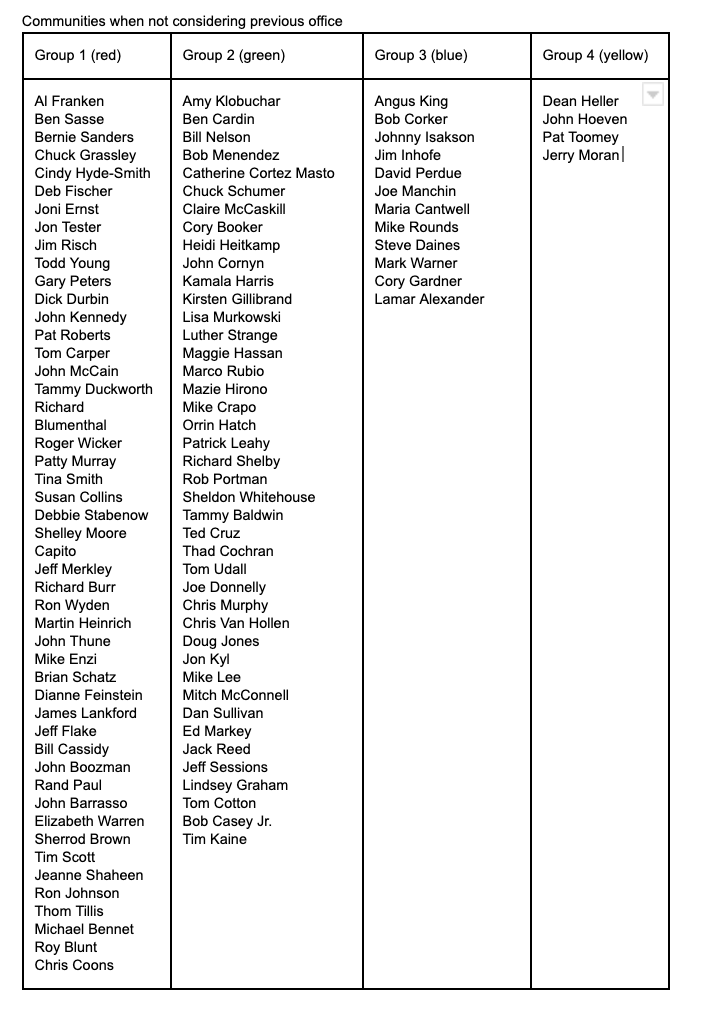
\includegraphics[width=3.2in]{comm_no_office}
    \caption{{Communities of Senators by career history when not considering previous office.\newline Group 1 is a mix of mostly professional, nonprofit and administrative careers. \newline Group 2 is characterized by careers that focus on law. \newline Group 3 is characterized by a mix of business and real estate careers. \newline Group 4 is characterized by careers that focus almost exclusively on fiance.}}
    \label{fig:ds}
\end{figure}

We will now examine each of the nine key votes that met our criteria for bipartisan votes with bipartisan dissent. Dissenting votes will have the following form: Name(group when considering office/group when not considering office)
\begin{enumerate}
\item
"Department of Defense and Labor, Health and Human Services, and Education Appropriations Act, 2019" (HR 6157)

Jeff Flake(2/1), Mike Lee(2/2) , Rand Paul(4/1), David Perdue(3/3), Bernie Sanders(1/1), Ben Sasse(2/1), Pat Toomey(2/4)

\item
"Energy and Water, Legislative Branch, and Military Construction and Veterans Affairs Appropriations Act, 2019" (HR 5895)

Jeff Flake(2/1), Kirsten Gillibrand(2/2), Ed Markey(2/2), Rand Paul(4/1), Elizabeth Warren(2/1)

\item
Consolidated Appropriations Act, 2018 (HR 1625)

John Barrasso(4/1), Cory Booker(2/2), Bill Cassidy(4/1), Bob Corker(2/3), Tom Cotton(2/2), Mike Crapo(2/2), Ted Cruz(2/2), Steve Daines(3/3), Mike Enzi(3/1), Joni Ernst(2/1), Dianne Feinstein(2/1), Deb Fischer(2/1), Jeff Flake(2/1), Cory Gardner(3/3), Kirsten Gillibrand(2/2), Chuck, Grassley(2/1), Kamala Harris(2/2), Ron Johnson(3/1), John Kennedy(1/1), James Lankford(2/1), Mike Lee(2/2), Ed Markey(2/2), Claire McCaskill(2/2), Jeff Merkley(3/1), Rand Paul(4/1), David Perdue(3/3), Jim Risch(2/1), Bernie Sanders(1/1), Ben Sasse(2/1), Dan Sullivan(2/2), Thom Tillis(2/1), Elizabeth Warren(2/1)

\item
The Bipartisan Budget Act of 2018 (HR 1892)

Michael Bennet(2/1), Cory Booker(2/2), Richard Burr(3/1), Maria Cantwell(3/3), Bill Cassidy(4/1), Bob Corker(2/3), Mike Crapo(2/2), Steve Daines(3/3), Mike Enzi(3/1), Dianne Feinstein(2/1), Jeff Flake(2/1), Kirsten Gillibrand(2/1), Chuck Grassley(2/1), Kamala Harris(2/2), Mazie Hirono(2/2), Ron Johnson(3/1), John Kennedy(1/1), James Lankford(2/1), Mike Lee(2/2), Ed Markey(2/2), Jeff Merkley(3/1), Rand Paul(4/1), Jim Risch(2/1), Bernie Sanders(1/1), Ben Sasse(2/1), Pat Toomey(2/4), Elizabeth Warren(2/1), Ron Wyden(3/1)

\item
Further Additional Continuing Appropriations Act, 2018 (HR 195)

Richard Blumenthal(2/1), Cory Booker(2/2), Catherine Cortez Masto(2/2), Dianne Feinstein(2/2), Kirsten Gillibrand(2/2), Kamala Harris(2/2), Mazie Hirono(2/2), Patrick Leahy(2/2), Mike Lee(2/2), Ed Markey(2/2), Bob Menendez(2/2), Jeff Merkley(3/1), Chris Murphy(2/2), Rand Paul(4/1), Bernie Sanders(1/1), Jon Tester(3/1), Elizabeth Warren(2/1), Ron Wyden(3/1)

\item
"A joint resolution making further continuing appropriations for fiscal year 2018, and for other purposes." (HJ Res 123)

Cory Booker(2/2), Ted Cruz(2/2), Joni Ernst(2/1), Kirsten Gillibrand(2/2), Kamala Harris(2/2), Mazie Hirono(2/2), Mike Lee(2/2), Ed Markey(2/2), John McCain(2/1), Jeff Merkley(3/1), Mike Rounds(3/3), Bernie Sanders(1/1), Ben Sasse(2/1), Elizabeth Warren(2/1)

\item
National Defense Authorization Act for Fiscal Year 2018 (HR 2810)

Bob Corker(2/3), Kirsten Gillibrand(2/2), Patrick Leahy(2/2), Mike Lee(2/2), Jeff Merkley(3/1), RandPaul(4/1), Bernie Sanders(1/1), Ron Wyden(3/1)

\item
Countering America's Adversaries Through Sanctions Act (HR 3364)

Rand Paul(4/1), Bernie Sanders(1/1)

\item
Countering Iran's Destabilizing Activities Act of 2017 (S 722)

Rand Paul(4/1), Bernie Sanders(1/1)
\end{enumerate}

Unfortunately, we do not see any communities in these dissenting votes that are over represented to a significant degree. While it is tempting to look at something like HJ Res 123 where $11/14 = 78\%$ Senators are from group 2 (when considering previous office), group 2 accounts for about $68\%$ of all Senators. When the sample is only$14$ votes, this is less than $2$ more the expectation of $9.52$. Another trick of the data is group 4 (when considering previous office) makes a decent percent of many dissenting votes while less then $4\%$ of Senators are in group 4, but this is due almost entirely to one man, Rand Paul, and only looks significant because of the relatively small numbers being dealt with. It would be hard to argue that a single eccentric Senator makes a trend.

While that didn't pan out, since we have the data, let's look at a few more measures to see if we can find any predictive effect of career archetype.

Of the nine votes, the following Senators appeared in the bipartisan minority in more than half of them:
Rand Paul(4/1), Bernie Sanders(1/1), Kirsten Gillibrand(2/2), Mike Lee(2/2), Jeff Merkley(3/1), Elizabeth Warren(2/1), Ed Markey(2/2). Again, there does not appear to be any over represented group hinting at a trend, and the numbers are small enough that even if there were, any argument would be weak.

We can easily find the group counter to that, those who never voted against the majority in the sampled votes, the following 59 Senators:

Susan Collins, Joe Donnelly, John Boozman, Marco Rubio, Doug Jones, Brian Schatz, Jon Kyl, Tom Udall, Lisa Murkowski, Johnny Isakson, Pat Roberts, John Cornyn, Shelley Moore Capito, Gary Peters, Debbie Stabenow, Tina Smith, Chris Coons, Dean Heller, Lamar Alexander, Jeanne Shaheen, Cindy Hyde-Smith, John Hoeven, Jack Reed, Maggie Hassan, Dick Durbin, Bill Nelson, Jerry Moran, Orrin Hatch, Roger Wicker, Chuck Schumer, Angus King, Amy Klobuchar, Lindsey Graham, Tammy Duckworth, Ben Cardin, Joe Manchin, Richard Shelby, Martin Heinrich, Tim Scott, Tim Kaine, Luther Strange, Jim Inhofe, Jeff Sessions, Al Franken, Chris Van Hollen, Mark Warner, Heidi Heitkamp, John Thune, Mitch McConnell, Roy Blunt, Rob Portman, Sherrod Brown, Tom Carper, Thad Cochran, Todd Young, Patty Murray, Tammy Baldwin, Bob Casey Jr., Sheldon Whitehouse

As we see in figure 5, there again does not seem to be a trend, each group is fairly evenly represented.
\begin{figure}[H]
    \centering
    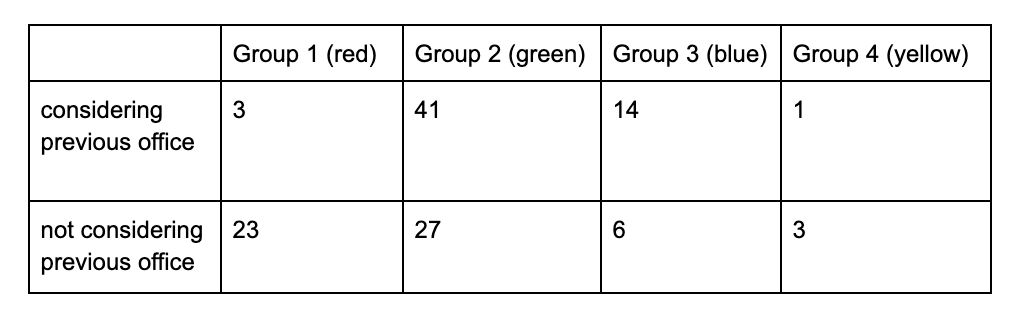
\includegraphics[width=3in]{major}
    \caption{Number of Senators who never vote against the majority in each group.}
    \label{fig:ds}
\end{figure}

Finally, let's look at career archetype and party affiliation. The numbers from figure 6 do show what look to be trends. Membership in group 4 when considering previous office is associated exclusively with Republicans, as is membership in group 4 when not considering previous office. These represent the medical and finance professions respectively. Though the numbers again are too small too make strong claims, there might be something there, it would worth looking into further in another study. We also see a slight trend towards Republicans in group 3 when not considering previous office, an archetype representing business with real estate which is interesting in that it goes against the slight trend towards Democrats in group 3 when considering previous office, business and professionals. This could hint at a bit of a hidden trend, professionals and Democrats and real estate and Republicans, but as always the data set is small and at some point we are just reading tea leaves.

\begin{figure}[H]
    \centering
    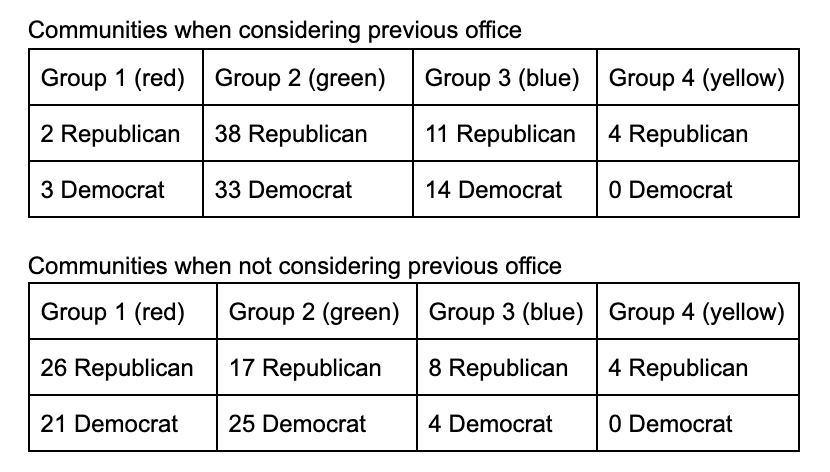
\includegraphics[width=3in]{rep_dem}
    \caption{Party affiliation within groups}
    \label{fig:ds}
\end{figure}

	\section{Discussion}
	While we did not find what we were looking for, career archetypes that are associated with bipartisan voting minorities, we did get something out of these results. We will discuss what trends seem to exist or not and what future work might be done with this knowledge.
	\subsection{Breakdown of Results}
	First, community detection by maximizing modularity did a respectable job of finding reasonable career archetypes. Even though there was no guarantee of sensible community structure, no real ground truth of what a community was, it found groups that have clearly interpenetrate results that pass a human sanity check. Even with the burden of nearly all Senators having held prior office, community detection was not overwhelmed. There are even interesting subtleties to some of the communities found, like how business and real estate is different from and trends towards a different party than business and professionals.
	
	In general, career archetypes did hint at party affiliation trends that seem true as someone who observes politics at a human perception level. Without more data it is hard to tell if they are truly true or significant, but it does point to something.
	
	Unfortunately the stated goal of this project, to find correlation between career archetypes and bipartisan voting patterns, did not play out. The results do not show any meaningful trend that suggests previous career choice means anything about how Senators vote. However, there are other ways to look at the same problem that might yield different results. For one, the job categorization was done entirely by human judgment. While I feel like a can defend the decisions made, these are not by any means objective and are open to challenge. Perhaps another way sorting jobs would show interesting trends. Similarly, the choice of what types of votes to examine was just human judgment. I explained how I came to this choice in the methods section, but there is nothing stopping another measure from being more revealing.
	
	Additionally, I did not present any sort of network style analysis on the relations formed by Senators' votes. While another co-voting community detention was done with this, it was my feeling that the numbers being dealt with were already small, making it hard to claim anything with confidence. Subdividing the dissenting votes into even smaller slots did not yield anymore interesting results, statistically at least. It's pretty readily observable from the data that Senators Bernie Sanders and Rand Paul voted together many times. It's fun to notice that a self-labeled socialist and self-labeled libertarian get paired together here, but you can't make much out of it in the bigger picture.
	
	With those caveats stated, it is my feeling that negative result of this study is not the fault of the study, but is a truth about the problem. After looking through all the Senators and their key votes, I doubt that there is a career history measure that would find any meaningful predictive power over bipartisan voting patterns. There are so many other, more direct factors at play that I feel are the underlying causes of why these votes get made the way they do. It would be surprising if career, which appears to be a fairly limited spectrum anyway, plays a real role.
	
	\subsection{Future Work}
	One obvious way to extend this work is to recreate it but with more data. What few trends were found couldn't really be explored because they were too small. The data set can be widened by adding past sessions of congress and/or considering the same measures for the House of Representatives. The House is probably the more interesting way to go. As the larger body that includes more oddballs and political newcomers, it seems to have more potential for previously unseen patterns to be found.
	
	A relatively small thing worth looking into is the apparent lean of medical professionals turned Senators to be Republican. While the rightward tilt of finance and real estate don't seem surprising, I would generally assume that doctors and surgeons are pretty politically neutral professions. I would be curious to see if this holds up or is just an outlier of this particular configuration of the Senate.
	
	Finally, the exact workings of community detention by maximizing modularity might be something to play with. By default, we return the communities that produce the absolute maximum modularity found, which makes sense, but, as we can see below, there are other modularity scores that are very close to it. To reuse a previous example, for HJ Res 123 there where $11/14 = 78\%$ Senators are from group 2, which we decided was not significant because group 2 accounted for $68\%$ of all Senators. However, if all those Senators from group 2 were actually all within a smaller group previously that was merged into group 2, that might have been significant. By checking the smaller communities from fewer mergers, some significant trend might fall out.
		
\begin{figure}[H]
    \centering
    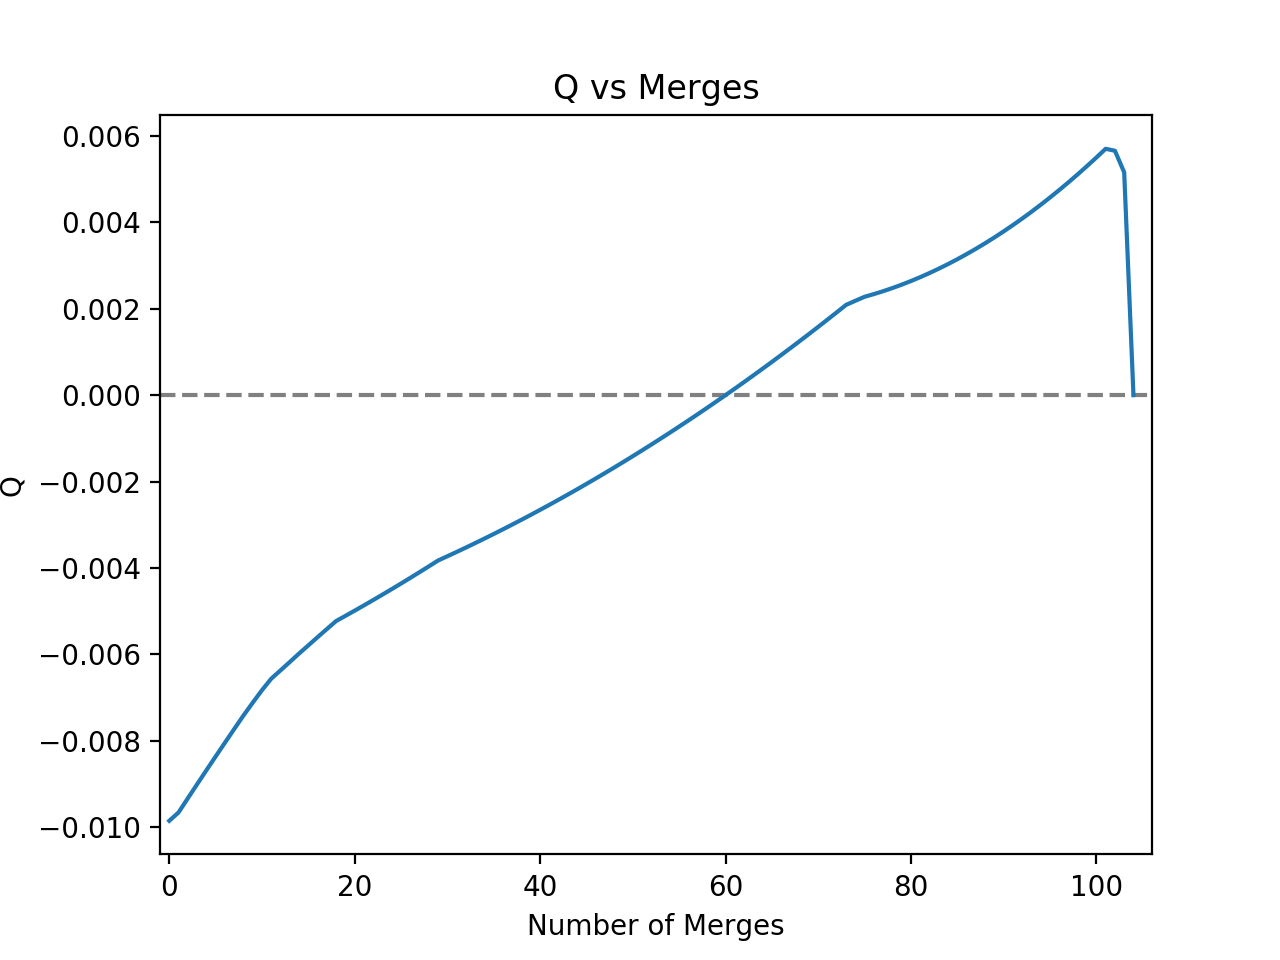
\includegraphics[width=2.2in]{qvm_w_office}
    \caption{Modularity score Q vs number of merges, considering previous office.}
    \label{fig:ds}
\end{figure}
\begin{figure}[H]
    \centering
    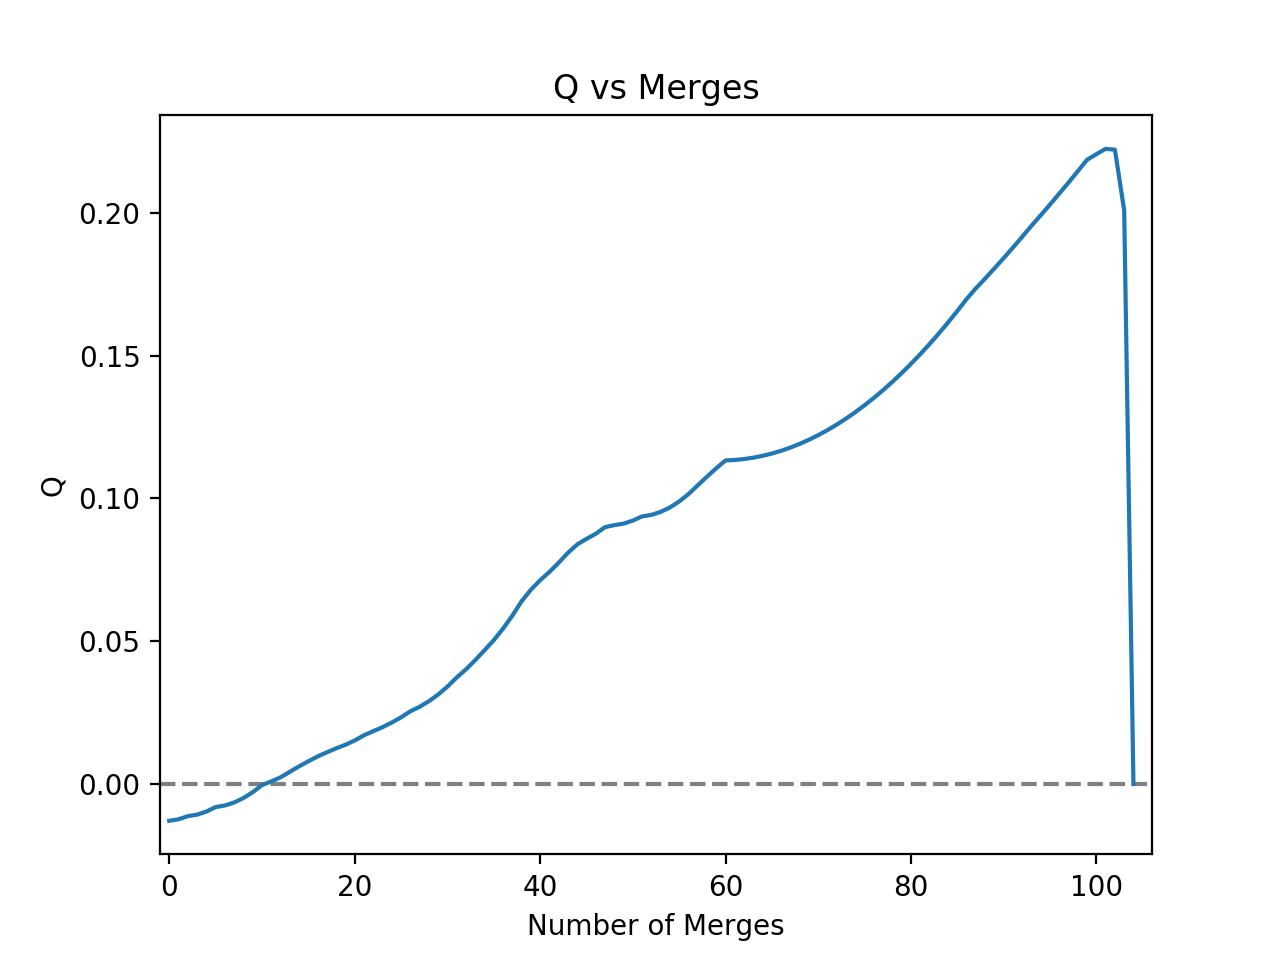
\includegraphics[width=2.2in]{qvm_no_office}
    \caption{Modularity score Q vs number of merges, not considering previous office.}
    \label{fig:ds}
\end{figure}
	\section{References}
	\subsection{Data Sources}
	\url{https://en.wikipedia.org/w/index.php?title=List_of_current_United_States_senators&oldid=875789149}
	
	\url{https://en.wikipedia.org/wiki/Jeff_Sessions}
	
	\url{https://en.wikipedia.org/wiki/Al_Franken}
	
	\url{https://en.wikipedia.org/wiki/Luther_Strange}
	
	\url{https://en.wikipedia.org/wiki/Thad_Cochran}
	
	\url{https://en.wikipedia.org/wiki/John_McCain}
	
	\url{https://ballotpedia.org/Key_votes:_115th_Congress,_2017-2018}
	
	\url{https://www.senate.gov/legislative/LIS/roll_call_lists/roll_call_vote_cfm.cfm?congress=115&session=2&vote=00212#position}
	
	\url{https://www.senate.gov/legislative/LIS/roll_call_lists/roll_call_vote_cfm.cfm?congress=115&session=2&vote=00207#position}
	
	\url{https://www.senate.gov/legislative/LIS/roll_call_lists/roll_call_vote_cfm.cfm?congress=115&session=2&vote=00063#position}
	
	\url{https://www.senate.gov/legislative/LIS/roll_call_lists/roll_call_vote_cfm.cfm?congress=115&session=2&vote=00031#position}
	
	\url{https://www.senate.gov/legislative/LIS/roll_call_lists/roll_call_vote_cfm.cfm?congress=115&session=2&vote=00017#position}
	
	\url{https://www.congress.gov/bill/115th-congress/house-joint-resolution/123/history?q=%7B%22search%22%3A%5B%22israel+aid%22%5D%7D}
	
	\url{https://www.senate.gov/legislative/LIS/roll_call_lists/roll_call_vote_cfm.cfm?congress=115&session=1&vote=00199#position}

	\url{https://www.senate.gov/legislative/LIS/roll_call_lists/roll_call_vote_cfm.cfm?congress=115&session=1&vote=00175#position}
	
	\url{https://www.senate.gov/legislative/LIS/roll_call_lists/roll_call_vote_cfm.cfm?congress=115&session=1&vote=00147#position}
	
	\subsection{Project Repo}
\bibliographystyle{abbrv}
\bibliography{refs}
\end{document}
